\pdfoutput=1
\documentclass[11pt]{article}
\usepackage{graphicx}
\usepackage{ACL2023}
\usepackage{verbatimbox}
\usepackage{times}
\usepackage{latexsym}
\usepackage{booktabs}
\usepackage[T1]{fontenc}
\usepackage[utf8]{inputenc}
\usepackage{microtype}
\usepackage{inconsolata}

\title{Faithful Benchmark for Information-Seeking Dialogue}

\author{Jagath Sai Narayana K \\
  University At Buffalo \\
  Buffalo, NY, USA\\
  \texttt{jagathsa@buffalo.edu} \\\And
  Siddhi Satish Jadhav \\
  University At Buffalo \\
  Buffalo, NY, USA\\
  \texttt{sjadhav3@buffalo.edu} \\\And
  Briyana Rana \\
  University At Buffalo \\
  Buffalo, NY, USA\\
  \texttt{brana@buffalo.edu}}

\begin{document}
\makeatletter\acl@finalcopytrue\maketitle
\begin{abstract}
As the demand for information-seeking dialogue systems increases, ensuring the accuracy and reliability of responses to user queries becomes crucial. When response utterances are not supported by underlying truth or ground knowledge, it can lead to negative consequences such as loss of trust in the system and a poor user experience. In domains like healthcare, finance, and education, the dissemination of false or misleading information can have severe implications. To address this issue, we propose a novel approach that focuses on generating knowledge-grounded responses based on conversation history and ground truth. By using this approach as a training signal, we aim to enhance the performance of existing dialogue systems. We introduce a hallucination critic that discerns between faithful and unfaithful responses, and we identify different Verbal Response Modes (VRM) to gain a comprehensive understanding of speech acts in dialogue. Additionally, we train a model to generate response utterances that align with the underlying knowledge sources, ensuring accuracy and reliability in information-seeking dialogue systems.
\end{abstract}

\section{Introduction}
Conversations lacking sufficient knowledge pose a significant challenge for information-seeking dialogue systems, which strive to deliver precise and reliable information to seekers. When responses are not firmly rooted in solid knowledge, seekers may receive incomplete or inaccurate information, leading to an erosion of trust in the system. Despite notable advancements in natural language conversation agents, the persistent issue of 'Hallucination' remains. Hallucination refers to the phenomenon where language models generate responses that seem plausible but lack a foundation in factual information or contextual understanding.\par
An illustrative example in Figure 1 showcases a dialogue between an open-source agent and an information seeker, where the agent mistakenly provides an incorrect response to a query about the largest state in the US, Texas instead of the correct answer, Alaska.
In order to tackle this challenge, our project adopts a systematic three-step approach. Firstly, we develop a Hallucination Critic, designed to discern the presence of hallucinated responses. Secondly, we establish a taxonomy of Verbal Response Modes (VRM), enabling us to gain a comprehensive understanding of the diverse speech acts occurring within dialogues. Lastly, we train a language model to generate responses that are firmly grounded in the underlying knowledge.\par
To accomplish this, we leverage the FaithDial dataset, which has been acquired from Wizards of Wikipedia on the HuggingFace platform. This dataset encompasses the complete conversation history, associated knowledge, original responses from the WoW agent, and meticulously annotated gold response data generated by human experts. By employing these invaluable resources and employing advanced techniques, our objective is to significantly enhance the accuracy and dependability of information provided by dialogue systems.
\begin{figure}[h!] 
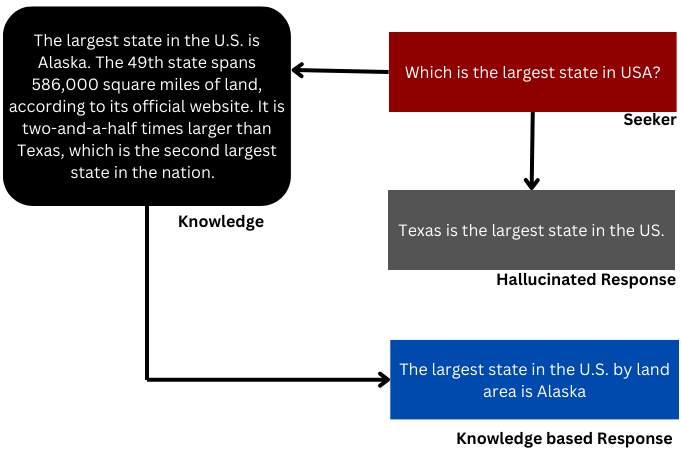
\includegraphics[scale=0.40]{AllImgs/High_diag.png}
\caption{High-level representation on the text generation}  
\label{fig:erd}
\end{figure}

\section{Related work}
The models being used in the current approach are BERT classifier and T5 text generation model. Although text generation models have shown impressive capabilities in generating text but, these models often suffer from hallucination, producing outputs that contain fabricated information. Following are the latest research and techniques aimed at addressing hallucination in text generation models as well as classification tasks. \par
"FAITHDIAL: A Faithful Benchmark for Information-Seeking Dialogue" by Dziriy et al. introduces a comprehensive benchmark dataset designed specifically for information-seeking dialogue systems. The authors highlight the issue of hallucination in existing benchmarks, which refers to the generation of unsupported utterances by dialogue systems. The main objective of this proposed dataset is to establish a benchmark that is free from hallucination, ensuring that all responses provided by the dialogue systems are firmly grounded on reliable knowledge sources.\par
"BERT for Multi-label Text Classification" by Sun et al. (2019):
 The paper introduced a hierarchical attention network that utilizes BERT embeddings to capture contextual information and hierarchical dependencies within the document. The model achieved competitive results on benchmark multi-label classification data sets, showcasing the effectiveness of BERT in this context.\par
"Plug and Play Language Models: A Simple Approach to Controlled Text Generation" by Dathathri et al. (2020):
The paper focused on controllable text generation using T5. They proposed a straightforward yet effective approach to modify T5's behavior by conditioning it on prompts and few-shot demonstrations. This technique empowered users to generate text with specific attributes or biases, allowing for greater control over the output.\par
"Exploring the Limits of Transfer Learning with a Unified Text-to-Text Transformer" by Raffel et al. (2019):
The paper introduced T5, a unified framework that achieved remarkable results across various NLP tasks, including text generation. The authors demonstrated the versatility of T5 by fine-tuning it on tasks such as summarizing, translation, and question-answering, achieving state-of-the-art performance.\par
\section{Data Description}
Faith-Dial is a benchmark data set specifically designed to provide hallucination-free or knowledge-grounded responses. Table 1 provides a description of the Faith Dial benchmark data set, including how the responses have been augmented to meet these criteria.

\begin{table*}
\centering
\begin{tabular}{lll}
\hline
\textbf{Dataset Label} & \textbf{Description} \\
\hline
Dialog idx & Id of the conversation\\
History & The conversation history \\
Knowledge & Ground truth based on which the response must be generated \\
Original Response & The response given by the agent without the knowledge \\
Response & The response given by the agent the knowledge\\
BEGIN & Begin labels for the wizard response\\
VRM & VRM labels for the wizard response\\
\hline
\end{tabular}
\caption{\label{citation-guide}
FaithDial dataset and description
}
\end{table*}

\section{Model Architecture}
The model is divided into three phases. The first phase is multiclass classification, where the task is to determine if the given text falls into the categories of "GENERIC," "UNCOOPERATIVE," "HALLUCINATION," or "ENTAILMENT" based on conversation history and knowledge. The second phase is multi label classification, which involves identifying if the given text belongs to the categories of "NONE," "ADVISEMENT," "QUESTION," "ACK," "EDIFICATION," or "DISCLOSURE" based on conversation history and knowledge. The third phase of the project focuses on text generation using a transformer model. Prior to performing all the phases, the data pre-processing step involves converting the list of history into a single string and then concatenating the newly created history with the knowledge.
\begin{figure}[h]
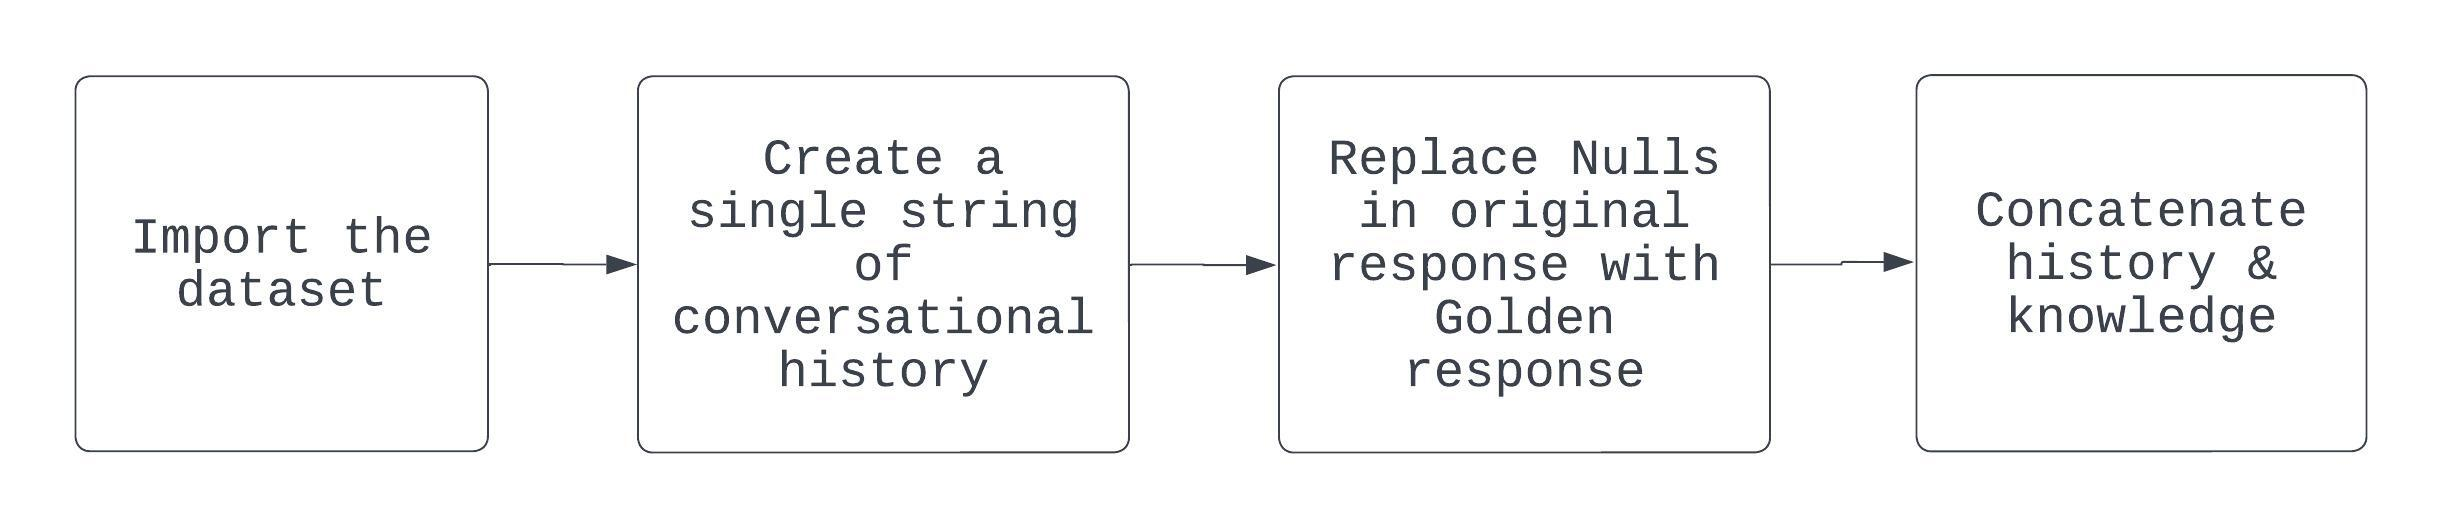
\includegraphics[scale=0.39]{AllImgs/Data_preprocessing.jpeg}
\caption{Data Pre-processing}  
\label{fig:erd}
\end{figure}

\subsection{Hallucination Critic}
As part of our approach, we build a Hallucination Critic to discriminate between faithful and unfaithful responses generated by dialogue systems. This task aims to improve response quality by filtering out unsupported responses and enhance the overall accuracy and reliability of the system. Once trained, the critic evaluates new dialogue system outputs, providing feedback to improve response quality. To achieve this we employ a BERT Multi-label classifier. This involves splitting the list of classes into different columns, encoding the tokens with special padding, and converting the data into tensors. We then encapsulate the entire dataset into a dataloader and pass it through the neural network. The model consists of the forward feed neural network, training, testing, and validation steps. These steps take the input IDs, attention mask, and labels as inputs and compute the loss using the Binary Cross Entropy function. The model uses the Adam optimizer to update its parameters and minimize the loss while maintaining the learning rates. The model is then trained for 2 epochs, and the best checkpoint is stored. The checkpoint is later loaded, and predictions are generated on the testing set. Table 2 and Figure 3 shows the count of classes, as well as a flowchart.

\begin{table}[h!]
\centering
\begin{tabular}{c c c c} 
 \hline
 Classes & Train & Test & Val\\ [0.5ex] 
 \hline\hline
 GENERIC & 116 & 32 & 23\\
UNCOOPERATIVE & 979 & 210 & 226\\
HALLUCINATION & 13507 & 2561 & 2525\\
ENTAILMENT & 15374 & 2679 & 2604 \\ 
 \hline
\end{tabular}
\caption{Begin Label count}
\label{table:1}
\end{table}

\begin{figure}[h]
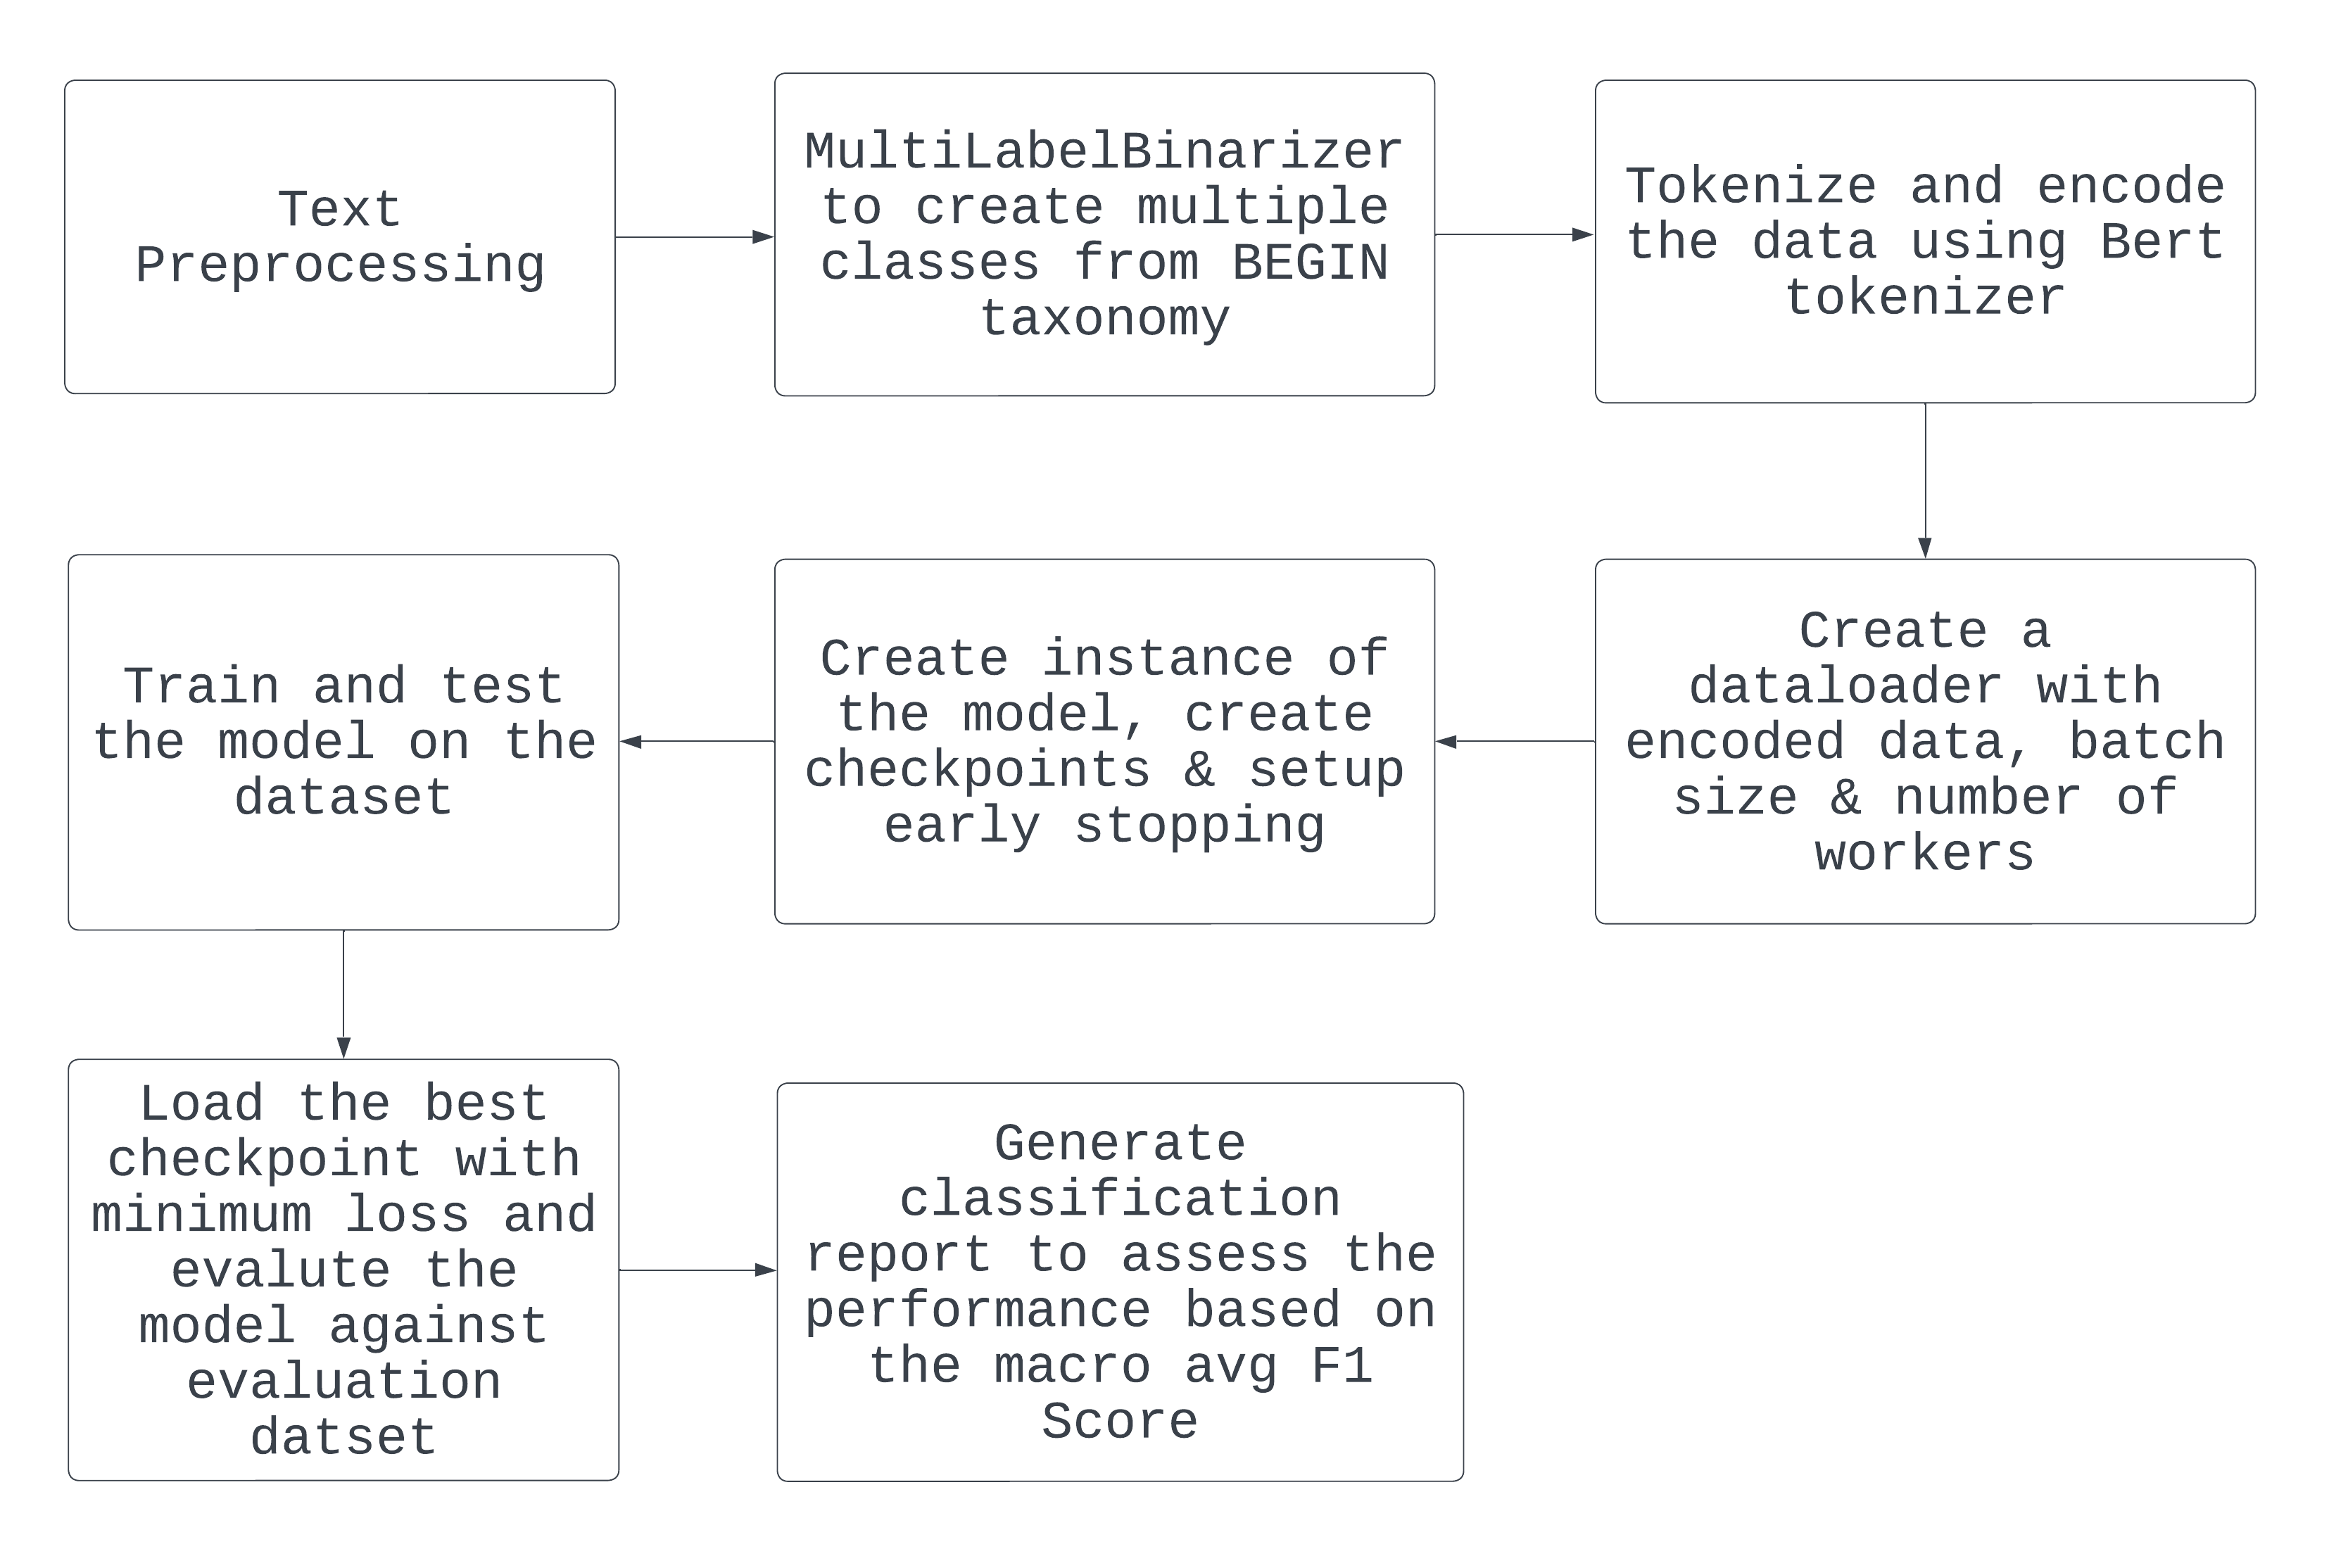
\includegraphics[scale=0.27]{AllImgs/Bert_Begin.png}
\caption{BEGIN classification Architecture}  
\label{fig:erd}
\end{figure}

\subsection{Multi-Class & Multi-Label Classification}
In the next phase of our approach, we focus on classifying the Verbal Response Modes (VRM) categories. By categorizing speech acts using VRM, we gain valuable insights into communication dynamics that can have diverse applications. Verbal response modes encompass the different ways speakers respond to verbal stimuli, such as questions, statements, or requests, and can be organized into distinct categories based on their function and structure. To achieve this we employ a BERT Multi-label classifier. This involves splitting the list of classes into different columns, encoding the tokens with special padding, and converting the data into tensors. We then encapsulate the entire dataset into a dataloader and pass it through the neural network. The model consists of the forward feed neural network, training, testing, and validation steps. These steps take the input IDs, attention mask, and labels as inputs and compute the loss using the Binary Cross Entropy function. The model uses the Adam optimizer to update its parameters and minimize the loss while maintaining the learning rates. The model is then trained for 2 epochs, and the best checkpoint is stored. The checkpoint is later loaded, and predictions are generated on the testing set.
\begin{table}[h!]
\centering
\begin{tabular}{c c c c} 
 \hline
 Classes & Train & Test & Val\\
 %[0.5ex] 
 \hline
 \hline
NONE & 55 & 12 & 7\\
ADVISEMENT & 565 & 1300 & 103\\
QUESTION & 2070 & 375 & 343\\
ACKNOWLEDGE & 7381 & 1303 & 1436\\
EDIFICATION & 10239 & 1878 & 1903\\
DISCLOSURE & 10587 & 2042 & 1928 \\ 
 \hline
\end{tabular}
\caption{VRM Label count}
\label{table:1}
\end{table}

\begin{figure}[h]
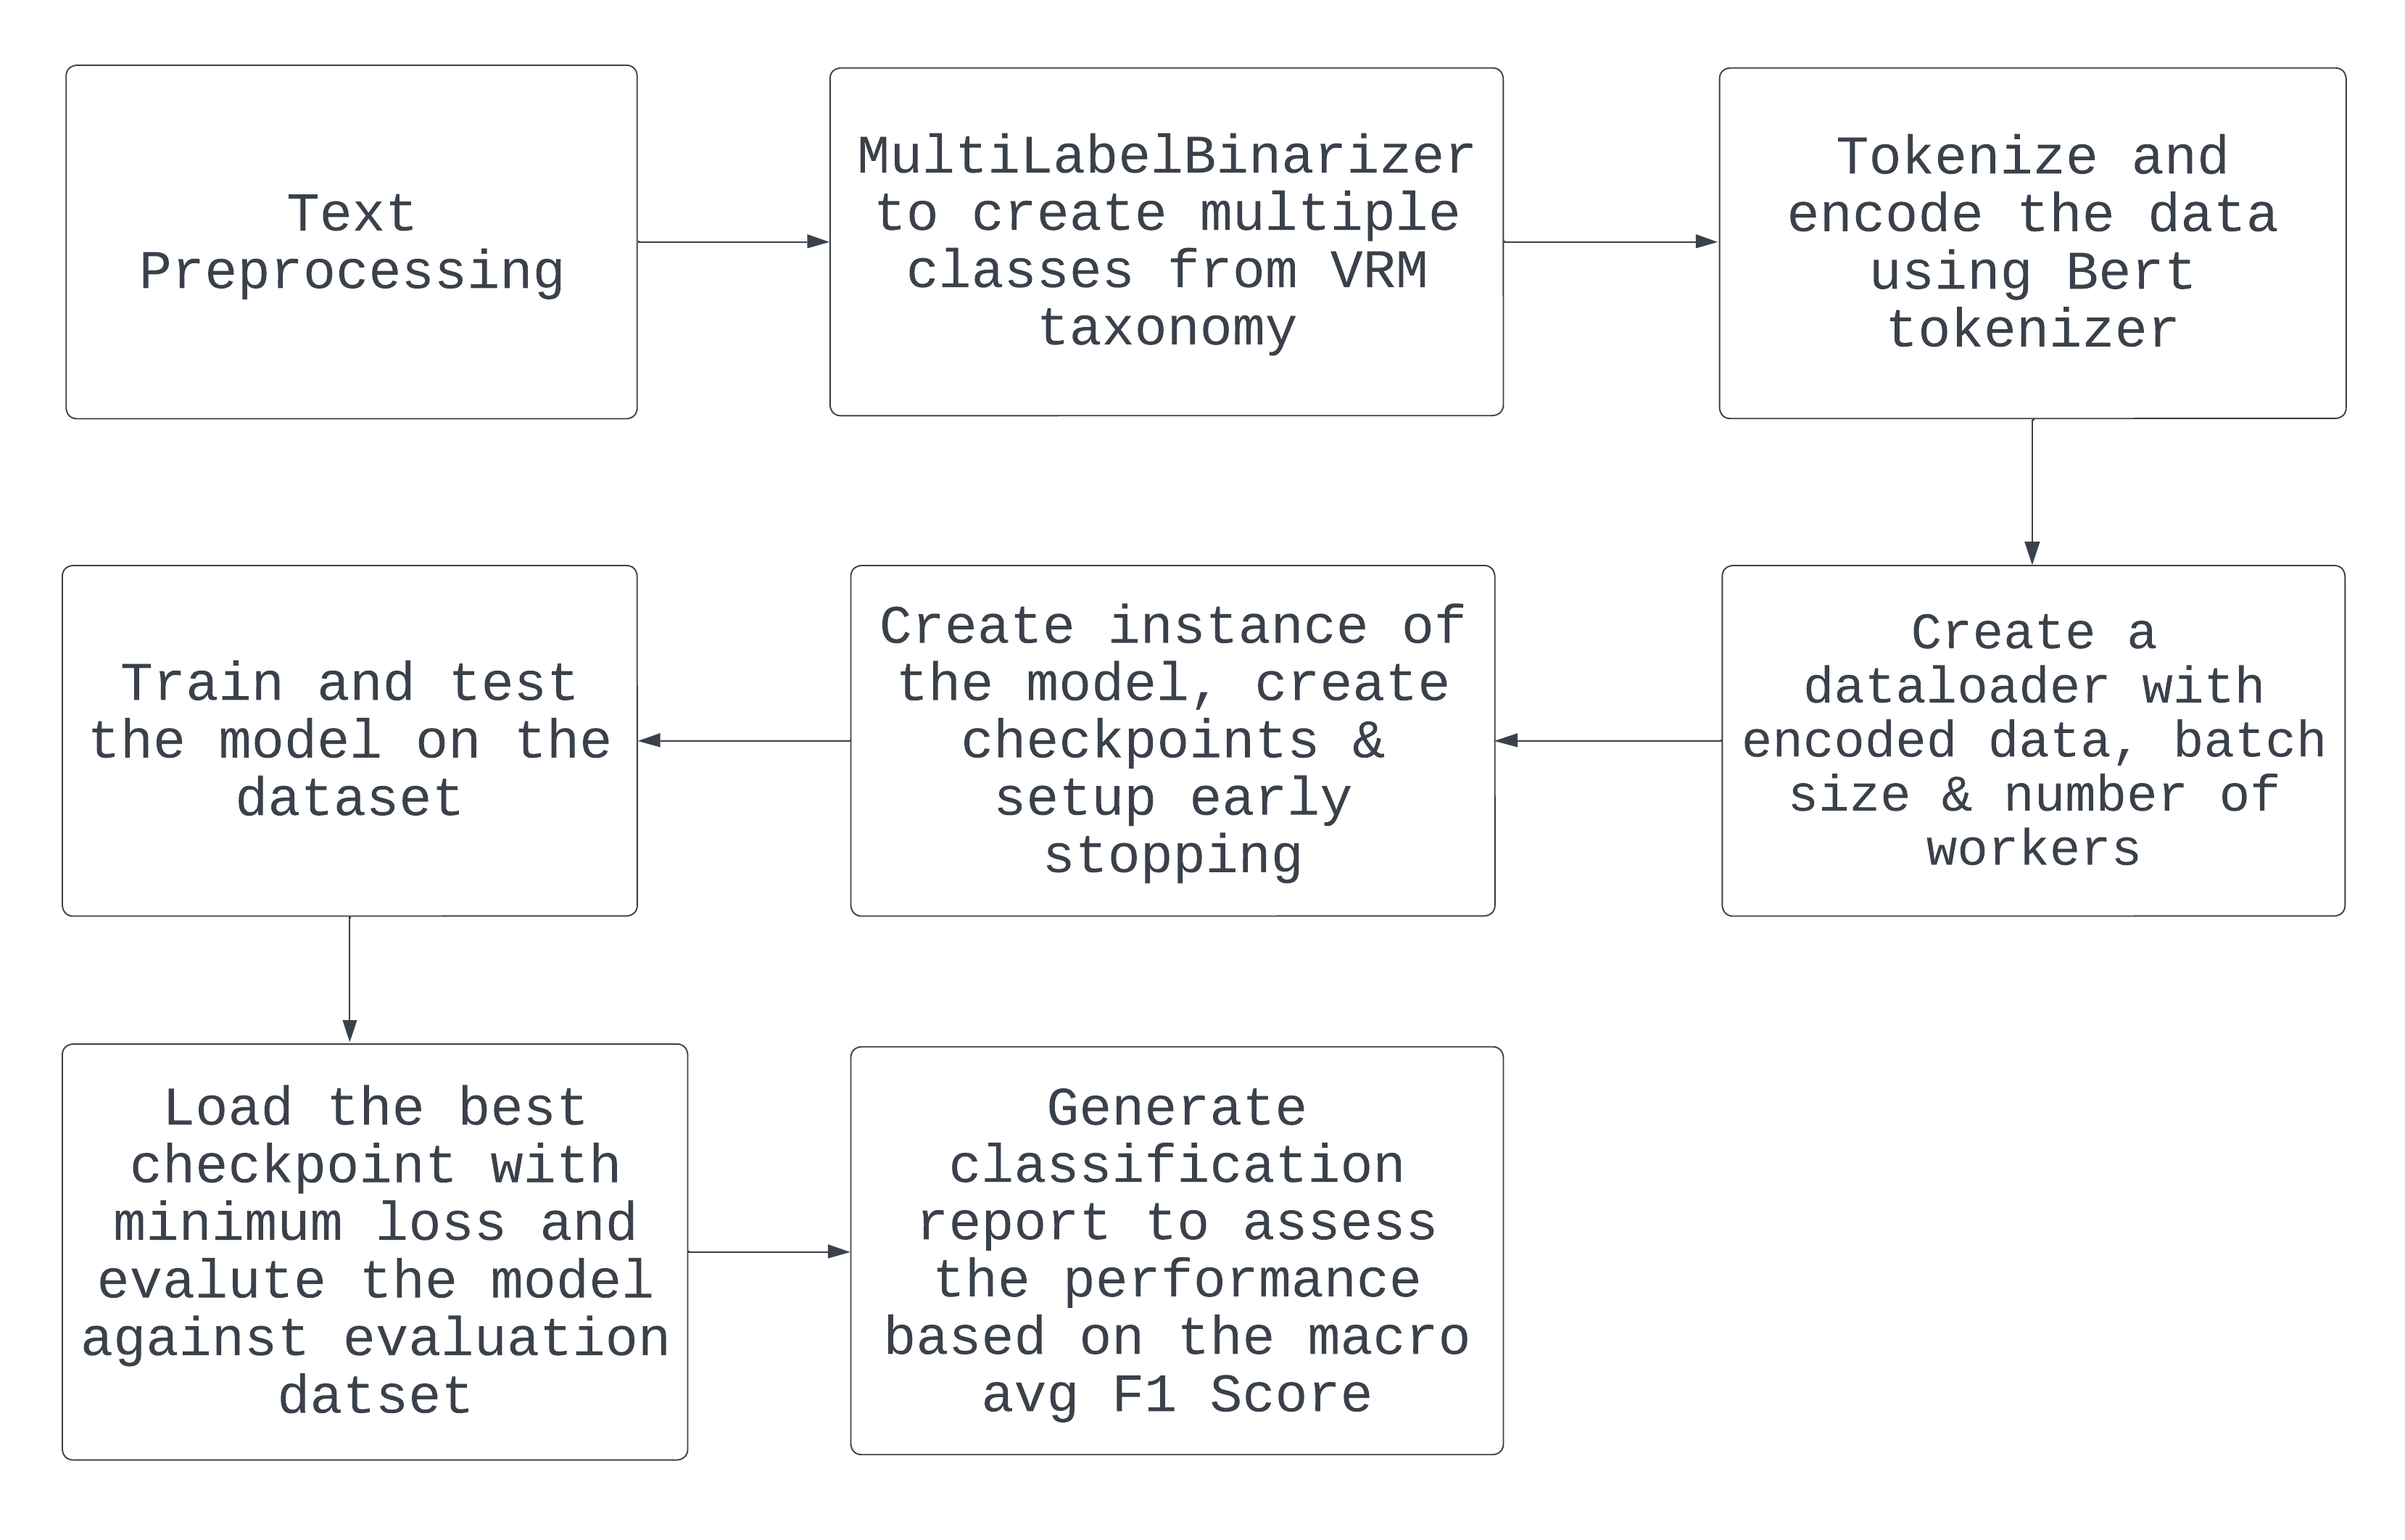
\includegraphics[scale=0.27]{AllImgs/Bert_VRM.png}
\caption{VRM classification Architecture}  
\label{fig:erd}
\end{figure}

\subsection{Text Generation}
The third phase is the actual task of generating hallucination-free text. To ensure the generation of coherent text data, we utilize the T5 transformer-based model. T5 is a versatile sequence-to-sequence model capable of performing text generation and text-to-text tasks, such as translation, summarization, and question-answering. Functioning as a fully conditional language model, T5 is trained to generate output sequences based on input sequences and control tokens. This characteristic makes it well-suited for text generatiom, where the model must generate appropriate responses. In the text generation task, we focus on three essential fields: conversation history, associated knowledge, and augmented or edited responses. To preprocess the data, we concatenate the conversation history and associated knowledge. Additionally, we extract the parts-of-speech tags from this concatenated string. Tokenization is then performed on the concatenated string, incorporating the parts-of-speech tags as control tokens in the source encoding. Target encoding is achieved by tokenizing the gold responses. The labels are derived from the target encoding, with padding tokens replaced by -100. After tokenizing the source and target, we create a data loader to handle the loading and processing of data for input to the T5 model, creating training, validation, and test sets. The T5 model is initialized with logging and early stopping enabled. It is then fine-tuned on the pre-trained T5 base model using the training set and validated using the validation set. The best model is saved, and its performance is evaluated on unseen test data. Finally, given the provided knowledge and conversation history, we aim to predict the model's generated response.

\begin{figure}[h]
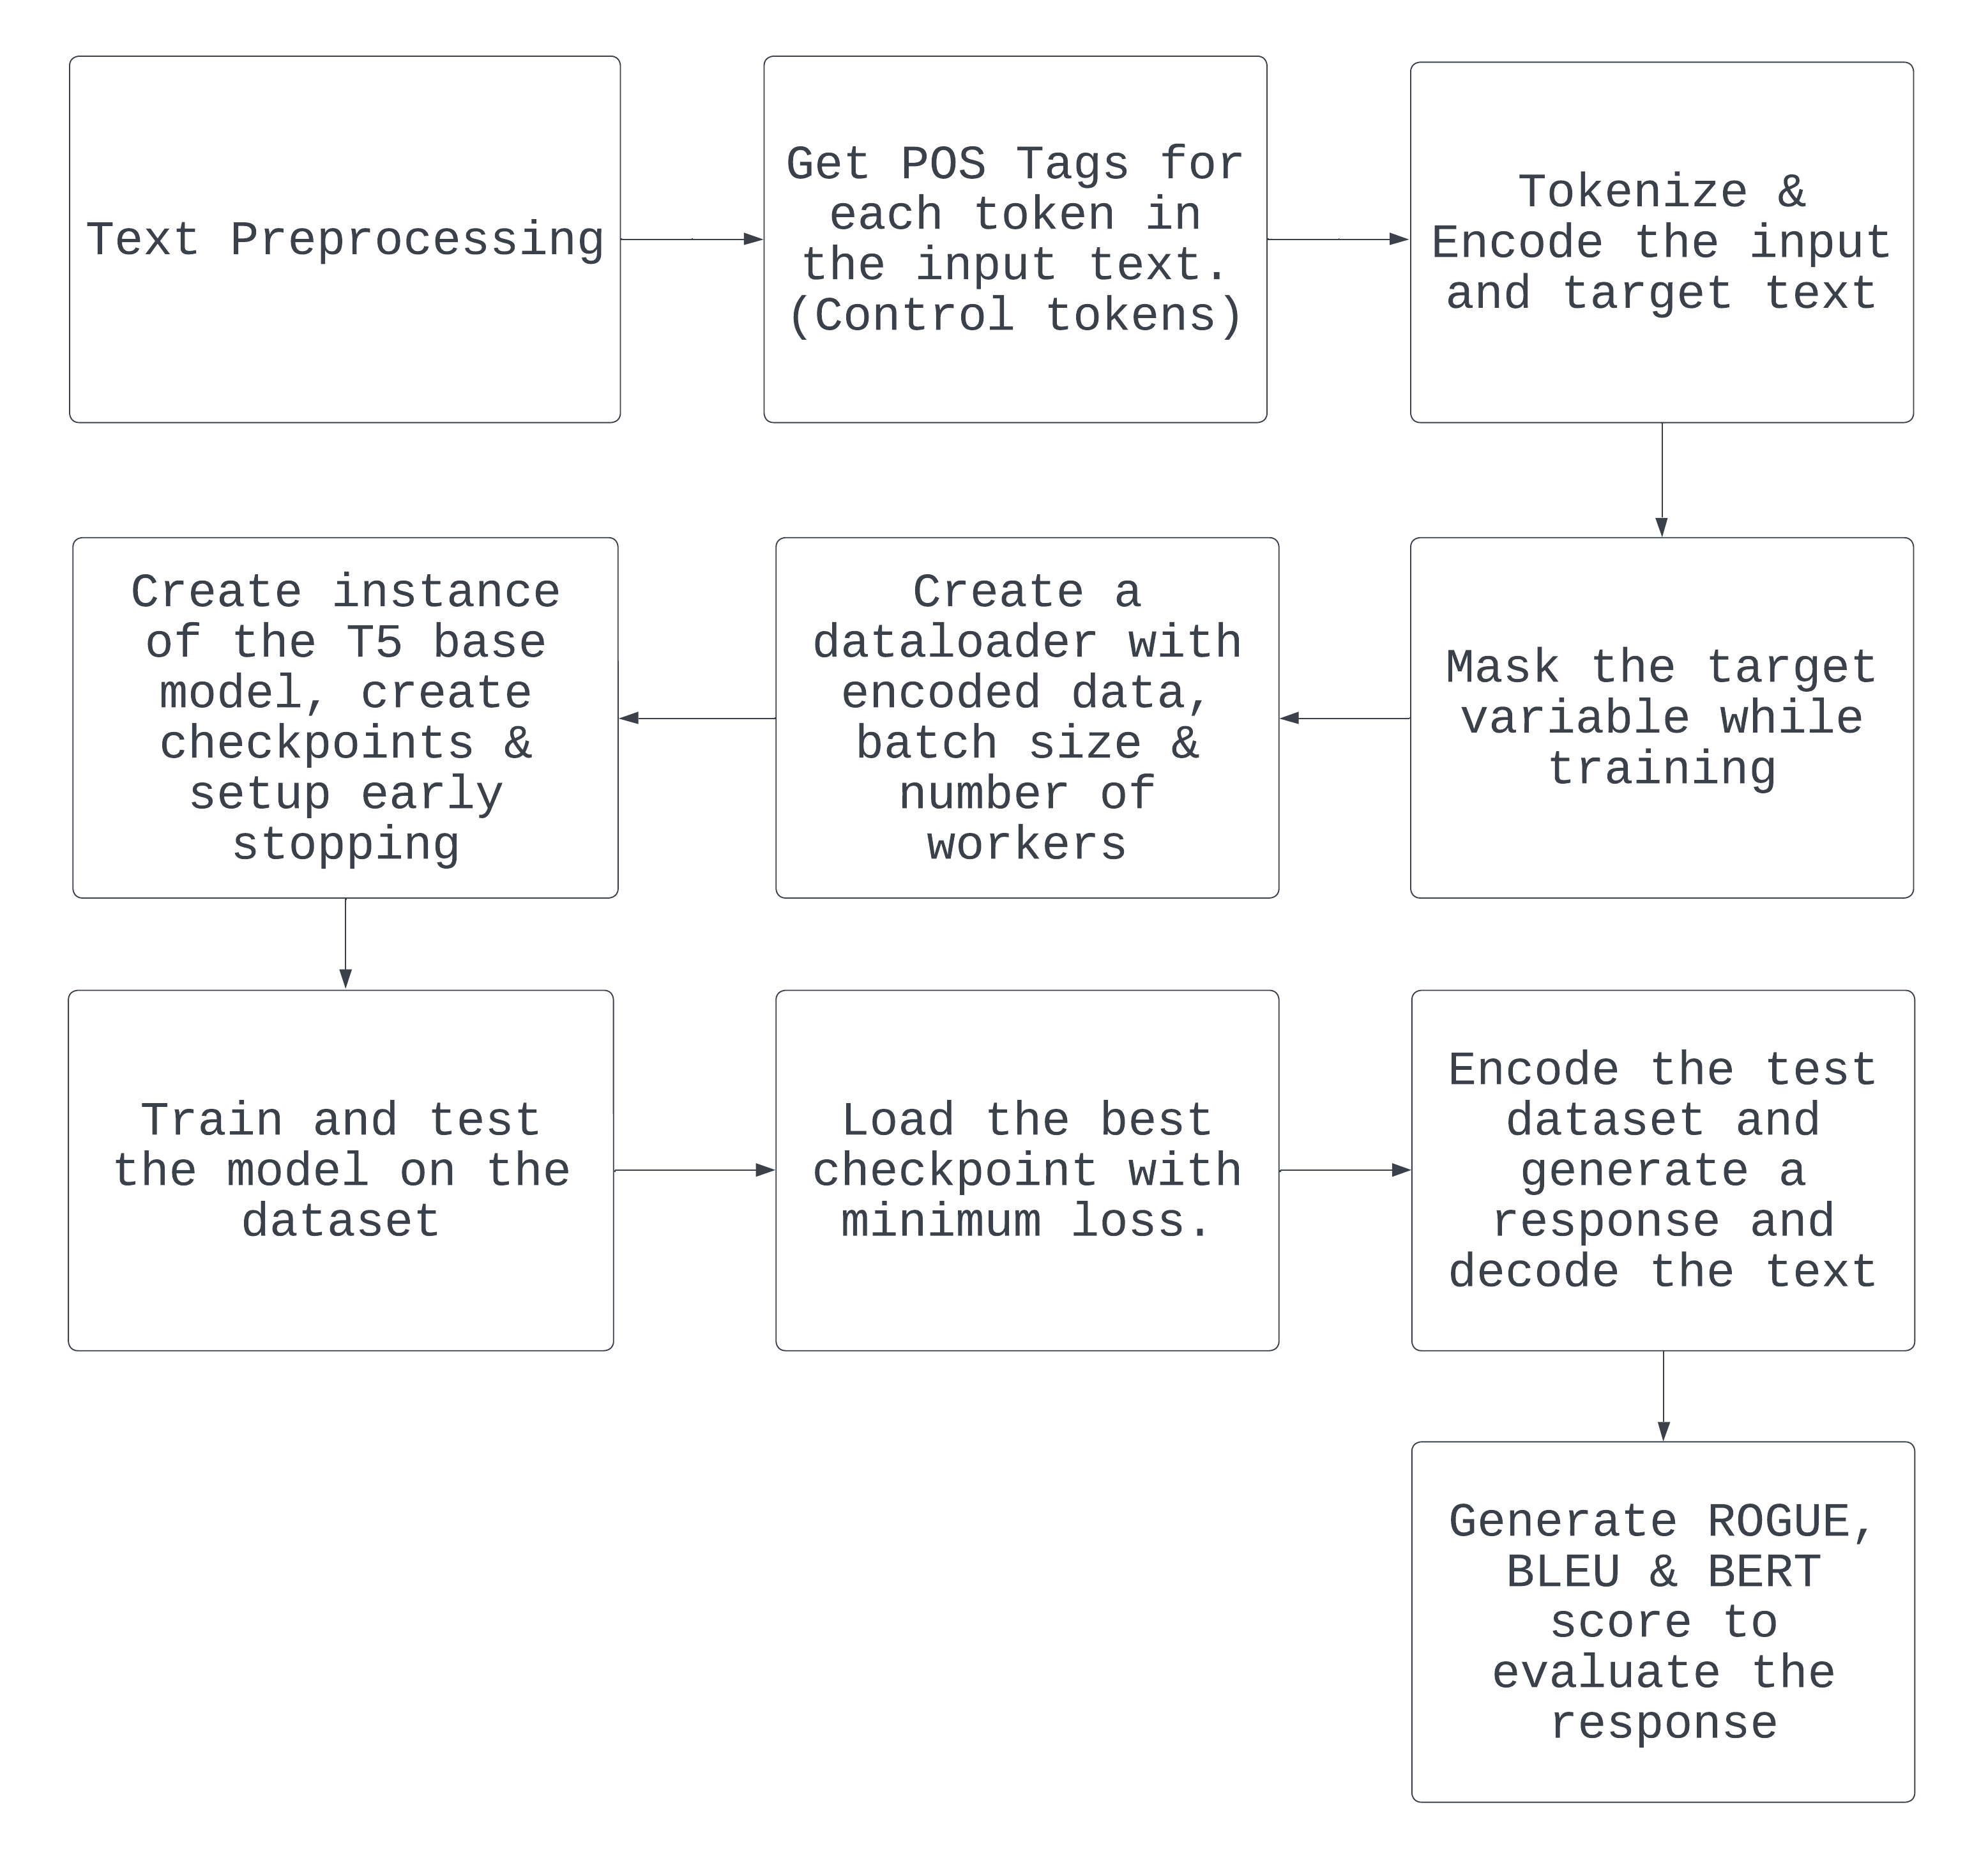
\includegraphics[scale=0.27]{AllImgs/text_gen.png}
\caption{Text Generation Model Architecture}  
\label{fig:erd}
\end{figure}

\section{Results}
\subsection{Hallucination Critic}
We initially implemented text classification using SVM, Multinomial Naive Bayes, and BERT for our baseline model. However, for the final architecture, we chose to proceed with BERT due to its ability to capture complex relationships and dependencies among words, which is advantageous for multi-label classification tasks. Furthermore, upon examining the data set, we observed a significant frequency imbalance between the 'Hallucination' and 'Entailment' labels compared to 'Edification' and 'Disclosure'. To address this issue, we utilized BERT's pre-training and fine-tuning approach, enabling the model to learn from the imbalanced distribution and adjust label probabilities, resulting in improved handling of imbalanced data. The classification report shows macro-average F1 scores of 0.42, 0.42, and 0.43 for SVM, MultinomialNB, and BERT, respectively, for the BEGIN taxonomy. However, the macro-average F1 score fails to consider the data set's class imbalance, treating all classes equally regardless of their size. In such cases, the F1 micro-average score is more appropriate as it provides a suitable metric for imbalanced data sets, where the performance on larger classes has a greater impact on the overall evaluation. Upon observing the micro-average F1 scores, we find that SVM, MultinomialNB, and BERT achieve scores of 0.81, 0.81, and 0.83, respectively. Clearly, BERT demonstrates the best overall performance among the models evaluated.
\begin{figure}[h]
\includegraphics[scale=0.5]{AllImgs/Begin_SVM.png}
\caption{Begin classification using SVM}  
\label{fig:erd}
\end{figure}
\begin{figure}[h]
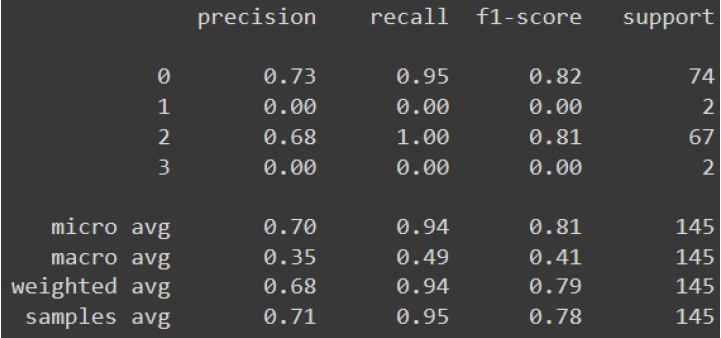
\includegraphics[scale=0.5]{AllImgs/Begin_naive.png}
\caption{Begin classification using MultinomialNB}  
\label{fig:erd}
\end{figure}
\begin{figure}[h]
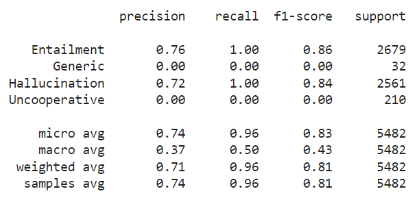
\includegraphics[scale=0.85]{AllImgs/Begin_Bert.png}
\caption{Begin classification using BERT}  
\label{fig:erd}
\end{figure}

\subsection{Multi-Label and Multi-class Classification}
We initially implemented text classification using SVM, Multinomial Naive Bayes, and BERT for our baseline model. However, for the final architecture, we chose to proceed with BERT due to its ability to capture complex relationships and dependencies among words, which is advantageous for multi-label classification tasks. Furthermore, upon examining the data set, we observed a significant frequency imbalance between the 'DISCLOSURE' and 'EDIFICATION' labels compared to 'ACKNOWLEDGEMENT', 'QUESTION', 'ADVISEMENT', and 'NONE'. To address this issue, we utilized BERT's pre-training and fine-tuning approach, enabling the model to learn from the imbalanced distribution and adjust label probabilities, resulting in improved handling of imbalanced data. The classification report shows macro-average F1 scores of 0.30, 0.34, and 0.33 for SVM, MultinomialNB, and BERT, respectively, for the VRM taxonomy. However, the macro-average F1 score fails to consider the data set's class imbalance, treating all classes equally regardless of their size. In such cases, the F1 micro-average score is more appropriate as it provides a suitable metric for imbalanced data sets, where the performance on larger classes has a greater impact on the overall evaluation. Upon observing the micro-average F1 scores, we find that SVM, MultinomialNB, and BERT achieve scores of 0.64, 0.58, and 0.60, respectively. Although SVM generates better results than BERT and MultinomialNB, considering the architectural benefits of BERT we choose to move forward with the same.
\begin{figure}[h]
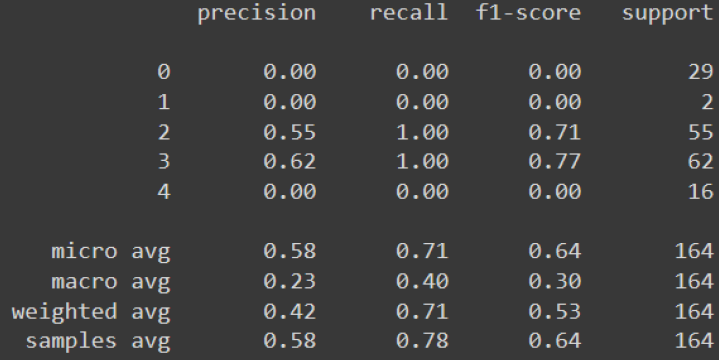
\includegraphics[scale=0.5]{AllImgs/VRM_Svm.png}
\caption{VRM classification using SVM}  
\label{fig:erd}
\end{figure}
\begin{figure}[h]
\includegraphics[scale=0.5]{AllImgs/VRM_naive.png}
\caption{VRM classification using MultinomialNB}  
\label{fig:erd}
\end{figure}
\begin{figure}[h]
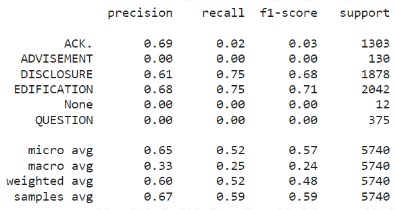
\includegraphics[scale=0.9]{AllImgs/VRM_Bert.png}
\caption{VRM classification using BERT}  
\label{fig:erd}
\end{figure}

\subsection{Text Generation}
Initially, for the text generation aspect of our approach, we constructed the model architecture using the GPT-2 transformer model. GPT-2 is a language model based on a transformer architecture, designed to understand natural language patterns and structure. However, despite its power, the transformer architecture has limitations and can struggle with certain inputs. GPT-2 generates text by predicting the probability distribution of the next word based on the preceding words, but it may encounter issues such as repetitive patterns and nonsensical output due to overfitting on the training data. When we applied the GPT-2 model for text generation, we encountered nonsensical and repetitive output, as illustrated in Figure 11. To address this problem, we opted for a more powerful transformer model, T5, for the final implementation. T5 proved to be superior in generating coherent sentences and avoiding hallucinations. To evaluate the model, we employed metrics such as ROUGE, BLEU, and BERT scores. We tested the model on an unseen test dataset, as shown in Figure 13, and obtained an average ROUGE score of 0.58, a better BLEU score of 0.38, and a high BERT f1 score of 0.89 when comparing the generated sentences to the gold responses. The scores for the entire test dataset can be found in Table 4. Additionally, we assessed the model's performance by manually providing seeker utterances and associated knowledge, as depicted in Figure 14. The model exhibited satisfactory performance in generating responses without hallucinations.
\begin{table}[h!]
\centering
\begin{tabular}{c c c} 
 \hline
 ROUGE1 & BLEU & BERT Score\\
 %[0.5ex] 
 \hline
 \hline
0.40 & 0.07 & 0.90\\
 \hline
\end{tabular}
\caption{Evaluation scores for the
entire test dataset}
\label{table:1}
\end{table}
\begin{figure}[h]
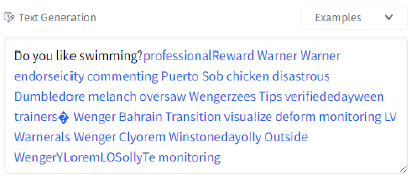
\includegraphics[scale=0.9]{AllImgs/GPT-2.png}
\caption{Text Generated using GPT-2} 
\label{fig:erd}
\end{figure}
\begin{figure}[h]
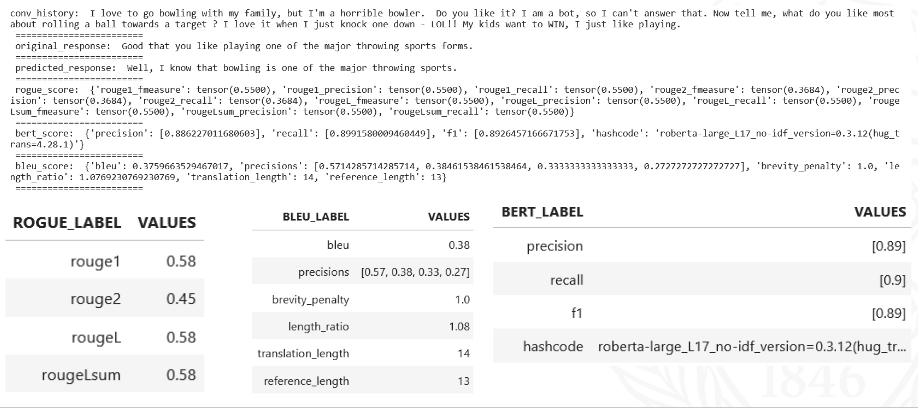
\includegraphics[scale=0.4]{AllImgs/T5_score.png}
\caption{Text generation and Evaluation using T5}  
\label{fig:erd}
\end{figure}
\begin{figure}[h]
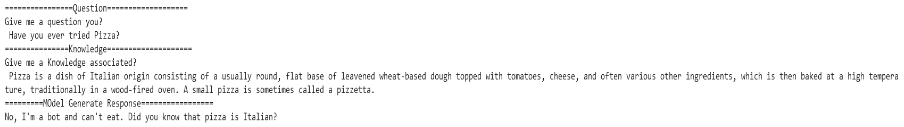
\includegraphics[scale=0.4]{AllImgs/Manual_text.png}
\caption{Manually text input}  
\label{fig:erd}
\end{figure}

\section{Discussion and Error Analysis}
From the baseline results, we were able to observe that we got low macro-average f1 scores due to highly imbalanced data set classes. To handle this, we can follow some other approach like data augmentation where we can generate some new examples for the underrepresented dataset or data up-sampling/down-sampling to have all the classes of the same distribution or use ensemble methods such as bagging or boosting that handle imbalanced data to improve performance, etc. Since the current dataset heavily relies on the knowledge provided by the user, we can use information retrieval methods to extract the knowledge data from Wikipedia based on the queries asked by the seeker. Besides that, we can utilize active learning techniques to improve the efficiency of dataset annotation and model training. We can also deploy the model as a conversational agent and collect user feedback to further improve the quality and naturalness of the generated responses.

\section{Conclusion}
We have successfully accomplished each task and generated hallucination-free responses based on the provided knowledge. However, due to the imbalance in label counts, we noticed significantly low scores, indicating an area that requires improvement. It is important to note that the accuracy and correctness of the generated text depend heavily on the quality and relevance of the knowledge being provided. Therefore, it is crucial to ensure that the knowledge is retrieved from reliable sources and kept up to date.

\section{Contribution}
Developed data pre-processing step involving creating a single string of history, replacing nulls, and concatenation of the history and knowledge. Implementation of TF-IDF, Multinomial Naive Bayes, and creating a pipeline for the second milestone. Implemented Bert classifier for BEGIN and VRM taxonomy. Converting Bert classifier into Pytorch Lighting and fine-tuning it. Implemented POS tagging as a control token in text generation.

\begin{table}[h!]
\centering
\begin{tabular}{c c c c} 
 \hline
 Task & Contribution\%\\
 \hline
 \hline
Hallucination Critic & 70\% \\
Multi-label \& class classifier & 70\% \\
Text generation & 20\% \\
 \hline
\end{tabular}
\caption{Contributions Table}
\label{table:1}
\end{table}

\nocite{dziri2022faithdial,raffel2020exploring, dathathri2020plug, chalkidis2020empirical, filippova-2020-controlled}
\bibliography{custom.bib}
\bibliographystyle{acl_natbib}

\appendix
\end{document}
